Il termine \textbf{``sicurezza"} si riferisce a tecnologie, processi e provvedimenti adottati per proteggere dati, reti di comunicazione, tecnologie informatiche e sistemi di calcolo da accessi non autorizzati o attacchi. \newline
L'approccio tradizionale prevede che la maggior parte delle risorse a disposizione per mettere in sicurezza il sistema si focalizzi sulle componenti più cruciali e che le protegga dalle minacce più grandi e più note; ovviamente ciò prevede che le componenti secondarie siano indifese e, inoltre, non protette da attacchi meno pericolosi. Tale approccio, però, risulta inefficiente nell'ambito della Smart Grid. \newline Per adattarsi al nuovo sistema, le organizzazioni promuovono un approccio più proattivo ed adattivo: il NIST, per esempio, ha recentemente pubblicato delle linee guida che consigliano uno spostamento verso il continuo monitoraggio e valutazioni real-time [ref].\newline \newline
La sicurezza della Smart Grid è un tema fortemente discusso, in relazione alla sua crescita: tutti concordano nel sostenere che la Smart Grid dovrebbe avere un modello di sicurezza robusto; il problema è che ci si trova a dover affrontare due sfide: come poter rispondere ai requisiti richiesti e come poter applicare le numerose alternative esistenti quando si cerca di rendere sicuro un ambiente complesso come la Smart Grid.
\newline \newline
Quando si sente parlare di ``nuova tecnologia", ``interconnessione", ``condivisione dei dati", subito ci si focalizza sui benefici e sulle nuove funzionalità che tali concetti portano con loro. C'è da considerare, però, anche i nuovi rischi che queste nuove funzionalità portano all'interno del sistema.\newline Per questo motivo, lo scopo della sicurezza è quello di garantire che le funzionalità del sistema operino correttamente e siano protette da abusi. È importante sottolineare, però, che non esistono applicazioni, reti o sistemi completamente sicuri e le Smart Grid non sono un'eccezione. Sebbene ogni componente della nuova rete elettrica porti con se numerosi miglioramenti operazionali  o funzionali, introduce anche nuove vulnerabilità e rischi addizionali che, se non propriamente gestiti, possono portare il sistema ad essere aperto ad attacchi.
\section{Cenni storici}

\section{Definire la sicurezza}
La sicurezza tradizionale fa affidamento sulla cosiddetta \textbf{CIA triad} [ref.], che ne costituisce il cuore. La CIA triad comprende tre concetti: confidentiality, integrity ed availability. \newline Una concezione più moderna, e più adatta all'ambiente della Smart Grid, prevede l'utilizzo del \textbf{Parkerian hexad}, proposto da Parker nel 2002 [ref.]. Tale modello propone, in aggiunta ai tre classici concetti precedenti, altri tre principi: control (o possesion), authenticity ed usability (o utility). \newline All'interno di questi sei pilastri, è possibile trovare tutti i problemi relativi alla Smart Grid.
\begin{figure}[h]\centering{
  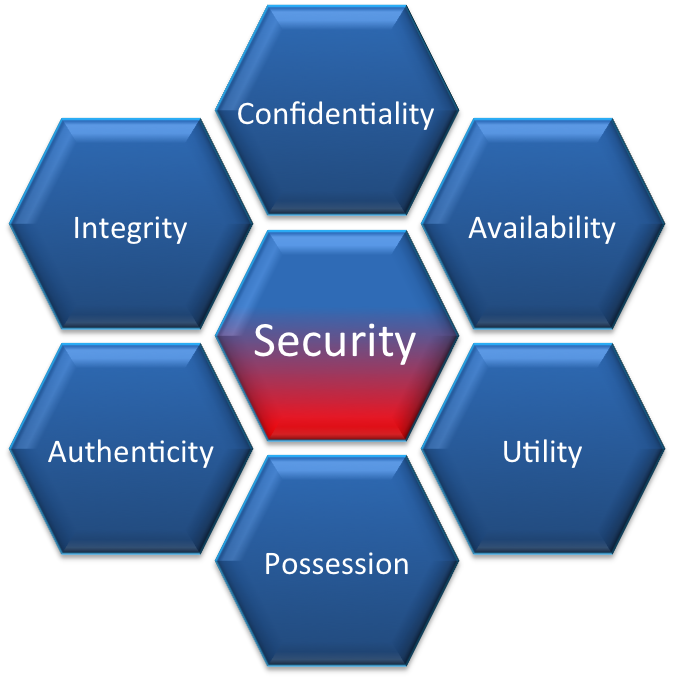
\includegraphics[scale=0.5, natwidth=674,natheight=679]{imgs/hexad.png}
  \caption{Parkerian hexad}
}
\end{figure}
\subsection{Confidentiality}
Tale concetto porta con sé una serie di problemi e di preoccupazioni connesse alla trasmissione e alla memorizzazione di dati ricavati dalle operazioni della Smart Grid. Questo tipo di dati, infatti, è spesso ritenuto \textit{confidenziale}, nel senso che se fossero noti, avrebbero tutto il potenziale per causare danni alla sicurezza delle operazioni di tutto il sistema. \newline La confidenzialità, inoltre, può essere intesa anche in un'altra accezione: se i dati fossero noti ad un concorrente, per esempio,  quest'ultimo potrebbe trarre vantaggio in uno specifico settore o in tutto il mercato. \newline A tali fattori si aggiungono altre problematiche nuove legate alla \textit{privacy del consumatore} e, quindi, dei suoi dati, che vengono fuori da meccanismi quali l'AMI. Gli utenti, infatti, si aspettano che i consumi relativi alle loro abitazioni private rimangano confidenziali; se così non fosse, la disponiblità di tali informazioni insieme alla capacità di fare data mining, avrebbe il potenziale per creare significative preoccupazioni sulla privacy. \newline I punti della Smart Grid che introducono rischi per la confidenzialità, sono costituiti da tutte le locazioni in cui sono memorizzati i dati e da tutti i meccanismi di trasmissione delle informazioni. Per quanto riguarda i dati memorizzati, questi potrebbero essere letti, copiati e distribuiti a soggetti diversi dai destinatari. Per quanto riguarda la trasmissione, invece, sia su reti private che su reti pubbliche come Internet, i dati potrebbero essere intercettati, copiati e distribuiti. \newline La soluzione a tali problemi risiede nelle funzioni di \textit{cifratura dei dati} e di \textit{controllo degli accessi}. Fornendo l'appropriato livello di cifratura delle informazioni, quest'ultime possono essere protette da chiunque non sia il diretto destinatario. \newline Il controllo degli accessi, prevede che i dati siano protetti da coloro che hanno l'autorizzazione per accedere al sistema ma che, allo stesso tempo, non hanno bisogno di tali dati per svolgere il loro lavoro.


\subsection{Integrity}

\subsection{Availability}

\subsection{Control}

\subsection{Authenticity}

\subsection{Usability}

\section{Building blocks}

\section{Minacce e loro impatto}

\section{Sforzo dello stato (?)}

\section{Compagnie}

\section{Servizi di terze parti}

